In order to understand the $\tilde{\Theta}(\sqrt{n})$ quantum
query complexity, it is mandatory to learn the logic behind the
trichotomy theorem \cite{trichotomy_not_andris} and its dependency on regular
languages and star-free languages.
After that, it will be necessary to presents the tools
that computer scientists have developed in order to
find new bounds on the quantum query complexity.
These tools can be group into 3 main categories:
reductions, algorithms, and adversary methods\cite{adversary_equivalence}.

\subsection{Quantum query for regular languages.}

In the article \cite{trichotomy_not_andris}, Aaronson, Grier and Schaeffer use
a really interesting algebraic characterization of regular languages based on
monoids and syntactic congruence. This definition was unknown to me and I spent
a lot of time on understanding it correctly.

\subsubsection{Regular languages}

Usually, the set of regular languages $\mathcal{R}$ on the alphabet $\Sigma$ is
defined as the smallest fixed point of the function $F$ that includes $\{\varnothing\} \cup
    \{\varepsilon\} \cup(\cup_{l\in\Sigma}\{l\})$. With $F$ being the function that computes
concatenations, unions, and Kleene stars:
\begin{align*}\label{eq:F}
    F(X) = & \{AB,\  \forall (A,B)\in X^2\}                                                   \\
           & \cup \{A\cup B,\ \forall (A,B) \in X^2 \}                                        \\
           & \cup \{A\cap B,\ \forall (A,B) \in X^2 \}\ \texttt{\color{gray!50}$\#$ optional} \\
           & \cup \{A^*,\ \forall A \in X \}.
\end{align*}

However in \cite{trichotomy_not_andris}, the more convenient way to characterize
regular languages is to use their algebraic characterization. More precisely,
for every regular language $L$ it exists a finite monoid $M$, a subset $S$ of this monoid,
and a monoid homomorphism $\delta$ from $\Sigma^*$ to $M$ such that the regular language is exactly
the pre-image of the subset $S$ by the monoid homomorphism $\delta$ (i.e. $\delta^{-1}(S)$).
Let's take apart this characterization: A monoid is a 3-tuple of a set M, an
internal associative binary operation and finally the identity element associated to the
operation. A monoid homomorphism is a map from a monoid to another that preserves the
operation and the identity. Now, to get every elements of the characterization, the first
step is to compute the syntactic monoid. The syntactic monoid is
obtained by dividing $\Sigma^*$ by the following equivalence relation called syntactic
congruence
\[x \sim_L y \Leftrightarrow \forall (u, v) \in \left(\Sigma^*\right)^2, (uxv \in L \Leftrightarrow uyv \in L).\]
This equivalence relation is a congruence relation as the equivalence class can be multiplied
(i.e. if $x\sim_L y$ and $u \sim_L v$ then $xu \sim_L yv$). With this syntactic monoid, it is
now possible to define a monoid homomorphism. For that it is sufficient to take the
homomorphism that map an element to its congruence class. Moreover, using a subset of the
syntactic monoid is sufficient as in a congruence class, none or every element of the class
is in $L$. Indeed, if $x \sim_L y$ then for all
$(u, v)$ in $\left(\Sigma^*\right)^2, (uxv$ in $L \Leftrightarrow uyv$ in $L)$ thus
$x$ in $L$ is equivalent to $y$ in $L$. So, it exists a subset of equivalent class that
represent every word of $L$ and no word not in $L$.
Now, the last hard things to show is that the syntactical monoid is of finite size\footnote{
    More precisely, the finiteness of the syntactic monoid is the main property that
    characterize every regular languages. A good intuition to understand is first that it
    is always possible to construct finite automata from a finite monoid. For the second way,
    it is more delicate but the work done by Brzozozowski, Szykula and Ye \cite[2018]{Brzozowski}
    summarized a lot of result on the influence of the size of the minimal automata size on
    the size of the smaller syntactic monoid.}.
Finally, every regular language can be recognized by finite monoid.

\subsubsection{Star-free languages}\label{ssec:starfree}

The set of star-free languages is a really well studied subset of the regular languages.
Its definition differs a little from regular languages' one as the Kleene star is replaced
by the complement operation (noted $\overline{L}$). So star-free languages are defined
as the smallest fixed point of the function F' (the function that computes concatenations, unions
and complements) and such that it includes
$\{\varnothing\} \cup \{\varepsilon\} \cup(\cup_{l\in\Sigma}\{l\})$.
This restriction does not imply that every star-free language is finite.
For example, $\Sigma^*$ can be written $\overline{\varnothing}$ and the
language on $\Sigma = \{1, 2, 3\}$ described with the regular expression
$\Sigma^*20^*2\Sigma^*$ can be written as following in the star-free way
$\overline{\varnothing}2\overline{\overline{\varnothing}\Sigma{\setminus}
        \{0\}\overline{\varnothing}}2\overline{\varnothing}$.

As for regular languages, it exists an algebraic characterization for star-free
languages. Let $M$ be a monoid, $M$ is said to be aperiodic if for every $x$ in
$M$ it exits a positive integer $n$ such that $x^n=x^{n+1}$. A theorem proved by
Schützenberger \cite{Schtzenberger1965OnFM} states that a language is recognized
by a finite aperiodic monoid if and only if it is star-free.

Good examples of star-free languages are the Dyck word languages with bounded
heights. First, it is easy to have a finite automaton that recognize Dyck word
of height at most $k$ by putting one state for each integer from 0 up to $k$.
However, the belonging to the star-free regular languages is more delicate to
prove. It has been done by an italian researcher in
\cite[1978]{dyck_height_bound_star_free}.

\subsubsection{Trichotomy theorem}

\begin{theorem}[Aaronson, Grier and Schaeffer \cite{trichotomy_not_andris}]
    Every regular language has a quantum query complexity
    \(0,\Theta(1), \tilde{\Theta}(\sqrt{n}),\) or \(\Theta(n) \)
    according to the smallest class that contains
    the language in the following hierarchy.
    \begin{itemize}
        \item Degenerate: One of the four languages \(\varnothing, \varepsilon, \Sigma^*\), or \(\Sigma^+\).
        \item Trivial: The set of languages which have trivial
              \footnote{A language $L$ is said to be trivial if and only if it exists 2 finite size alphabets
                  $L_1$ and $L_2$ such that $L = L_1 \Sigma^* L_2$.}
              regular expressions.
        \item Star-free: The set of languages which have star-free regular expressions.
        \item Regular: The set of languages which have regular expressions.
    \end{itemize}
\end{theorem}

This theorem is really important as it gives a good idea for the quantum
query complexity of many language recognitions. Moreover, the classes are
now clearly defined so it is easier to know where is a problem compared
to the first classification describes in the introduction. However, it
does not give the exact quantum query complexity of every problem because,
as said in the introduction, the result for star-free languages is given
using a tilde $\thicksim $. The $\tilde{\Theta}(\sqrt{n})$ means that the
quantum query complexity of any star-free regular language is in
$\Theta(\sqrt{n}(\log_2(n))^{c_{te}})$ for some ${c_{te}}$ a non
negative constant. As it is known that for every $k$, \Dyck{k} is star-free\cite{dyck_height_bound_star_free},
it becomes an interesting problem to find the power of $\log_2(n)$ depending
on the value of $k$.

\subsection{The bounds for \Dyck{k} problem}

The trichotomy theorem state that for every $k$, \Dyck{k} language has
a quantum query complexity in $\tilde{\Theta}(\sqrt{n})$. The $\Theta$
means that the best possible algorithm is both a $\tilde{O}(\sqrt{n})$
and a $\tilde{\Omega}(\sqrt{n})$. So, a common method to find the power
of $\log_2(n)$ depending on $k$ is the squeeze theorem. More precisely,
the quantum query complexity of \Dyck{k} is trapped between a lower
and an upper bound for the quantum query complexity. So it is possible
to deduce the quantum query complexity from an increasing sequence of
lower bounds and a decreasing sequence of upper bounds such that they
share the same limit $l$ with $l$ equals to $Q(\Dyck{k})$. How to find
this sequence?
\begin{itemize}
    \item \textbf{For the lower bounds sequence.} Some of the most
          important tools to compute lower bounds are called
          \textbf{quantum adversary methods} and have been invented
          by Andris Ambainis \cite{andris_adversary_methode}. This
          tools can compute lower bounds more or less tight and some
          of this adversary methods have really useful property such
          as being compatible with a certain type of compositions
          of problems. This lead to the \textbf{reduction methods}
          that allow compute  a lower bounds from lower bounds of
          different but easier problems.
    \item \textbf{For the upper bounds sequence.} The main method
          is to \textbf{find quantum query algorithms} that are
          more and more efficient. An other way is also \textbf{by
              reduction} to a more difficult problem which has a good
          enough upper bound.
    \item \textbf{For the same limit.}
          The idea is to do an iterative process where each step
          improves successively each bound until only one will
          continue to be improved. Finally, both bounds may end
          up matching. However, before my internship, both lower
          and upper bounds for \Dyck{k} were respectively stuck
          to $\Omega\left(c^k\sqrt{n}\right)$ for some
          constant $c$ greater than 1 and
          $O\left(\sqrt{n}\left(\log_2(n)\right)^{0.5k}\right)$.
\end{itemize}


\subsubsection{Lower bounds on the quantum query complexity of \Dyck{k}}

\paragraph*{\textbf{The quantum adversary methods:}}
This part presents some quantum adversary methods and their usages.

\subparagraph*{\textbf{The adversary method.}} The classical adversary
method is a way to prove lower bound in classical algorithmic. Indeed,
the idea behind the classical adversary is to prove that for every
algorithm, it exist an entry such that the algorithm cannot decide
this entry in less unit of complexity than the lower bounds. In general,
during the algorithm execution, the adversary modifies values of the entry
that have not been already used in order to increase the execution time.
This classical adversary works great for classical algorithm but is not
really useable on quantum algorithms.

\begin{figure}[h!]
    \centering
    $
        \Qcircuit @C=.8em @R=1em {
        \lstick{\vdots} & \qw & \multigate{2}{U_0}  & \multigate{2}{Q} & \multigate{2}{U_1} & \qw &  & &  \multigate{2}{Q} & \multigate{2}{U_T}& \qw & \vdots& & \multigate{2}{\metersymbol{.2}} & \cw\\
        &\lstick{\ket{\psi_{start}}} qw & \ghost{U_0} & \ghost{Q} & \ghost{U_1} & \qw & \cdots & & \ghost{Q} & \ghost{U_T} &\qw & \ket{\psi_v^T} & &  \ghost{\metersymbol{.2}}& \cw\\
        \lstick{\vdots}& \qw & \ghost{U_0} & \ghost{Q}  & \ghost{U_1} & \qw & & &\ghost{Q} &\ghost{U_T}& \qw & \vdots & &\ghost{\metersymbol{.2}}& \cw \\
        }$
    \caption{Recall on the  structure of a quantum query algorithm.}
\end{figure}

\subparagraph*{\textbf{The super basic quantum adversary method.}}
In order to recognize a language it is mandatory to be able to
distinguish between a valid word $v$ and an invalid word $w$.
So before the measure at the end of the quantum query algorithm,
the states $\ket{\psi^T_v}$ and $\ket{\psi^T_w}$ should be
distinguishable, thus $\vert \langle \psi_v^T \vert \psi_w^T
    \rangle \vert < \frac{2}{3}$. How do they will differ? The
quantum query algorithm starts with $\ket{\psi^0_v} = \ket{\psi^0_w}
    = \ket{\psi_{start}}$. Moreover, the inner product
of both states isn't affected by $U_i$ gates because they are unitary
independent of $v$ and $w$. However, the $Q$ gates affect this
inner product as the behavior of each gate $Q$ is depending on the input.
Let's define the progress measure $\mathcal{P}$ such that $\mathcal{P}(t)
    := \langle \psi_v^t \vert \psi_w^t \rangle$ where $\ket{\psi^t_v}$
represents the quantum state after $U_t$ on the entry $v$. Let's suppose
it exists $d$ such that for all $0\leq t \leq T-1$,
$\vert \mathcal{P}(t+1)-\mathcal{P}(t)\vert \leq d$.
It implies the following inequality
\begin{align}
    \mathcal{P}(T) = \underbrace{\mathcal{P}(0)}_{=1} +
    \sum_{i=0}^{T-1}\underbrace{\mathcal{P}(i+1)-\mathcal{P}(i)}_{\geq -d}
    \geq 1 - T\times d.
    \label{eq:1}
\end{align}
Moreover, $\mathcal{P}(T)$ should be lower than $\frac{2}{3}$ so it
implies that $1 - T\times d$ should also be lower than $\frac{2}{3}$
and finally that $T$ should be a $O(\frac{1}{d})$. This gives a general
idea about how to determined a lower bound but it isn't precise enough
to get a theorem. In its courses, Ryan O'Donnell \cite{Odonnel_course}
explained a simple to understand adversary method called the super
basic adversary method. This adversary allows to compute a lower bound
by using the following method:

\begin{theorem}
    Let's define $YES$ the set equal to $f^{-1}(accepted)$ and $NO$ the set
    equal to \\ $f^{-1}(rejected)$. If it exists two subsets $Y\subseteq YES$ and
    $Z \subseteq NO$ such that:
    \begin{itemize}
        \item For each $y$ in $Y$, there are at least $m$ strings $z$ in $Z$ with dist$(y,z)=1$.
        \item For each $z$ in $Z$, there are at least $m'$ strings $y$ in $Y$ with dist$(y,z)=1$.
    \end{itemize}
    Then the quantum query complexity $Q(f)$ is in  $\Omega(\sqrt{m m'})$.
\end{theorem}


The proof of the theorem (adapted to the definition of the quantum query
circuit of the report) is detailed in \autoref{proof:advmethod}.
One important result of the adversary method is the lower bound on
the quantum query complexity of $Ex_{2m}^{m \vert m+1}$ in
$\Omega\left(m\right)$. The $Ex_{2m}^{m\vert m+1}$ problem consists in
recognizing between $|x|=2m\ \land\ |x|_1 = m$ , and $|x|=2m\
    \land\ |x|_1 = m+1$. More generally, an adversary method define
a process to find the lower value of $d$ possible  as lowering $d$
directly increase the lower bound on the quantum query complexity
(\autoref{eq:1}). The super-basic adversary method as its name let
suggests is simple but does not give a tight lower bounds for
many problems. Two more interesting but more complex quantum adversary
methods are now presented:

Let $f:D\to\{0,1\}$ be the function whose quantum query complexity is unknown.
\begin{itemize}
    \item \textbf{The Basic adversary method by Ambainis \cite{andris_adversary_methode}}.
          \begin{theorem}
              \label{th:basicadv}
              Let's define $YES$ the set equal to $f^{-1}(accepted)$ and $NO$ the set
              equal to \\ $f^{-1}(rejected)$. Moreover, let $Y\subseteq YES$, $Z \subseteq NO$, and
              let $\mathcal{R} \subseteq Y\times Z$ be a set of "hard to distinguish" pairs, such that:
              \begin{itemize}
                  \item For each $y$ in $Y$, there are at least $m$ strings $z$ in $Z$ with $(y,z)$ in $\mathcal{R}$.
                  \item For each $z$ in $Z$, there are at least $m'$ strings $y$ in $Y$ with $(y,z)$ in $\mathcal{R}$.
              \end{itemize}
              Also, let's define $\mathcal{R}_i$ as a restriction from $\mathcal{R}$ such
              that $(y, z)$ is in $\mathcal{R}_i$ if and only if $(y, z)$ is in $\mathcal{R}$
              and $y_i \neq z_i$.
              In addition,
              \begin{itemize}
                  \item For each $y$ in $Y$ and $i$, there are at most $l$ strings $z$ in $Z$ with $(y,z)$ in $\mathcal{R}_i$
                  \item For each $z$ in $Z$ and $i$, there are at most $l'$ strings $y$ in $Y$ with $(y,z)$ in $\mathcal{R}_i$
              \end{itemize}
              Then the quantum query complexity $Q(f)$ is in  $\Omega(\sqrt{\frac{m m'}{ll'}})$.
          \end{theorem}
    \item \textbf{The general adversary method by Reichardt \cite{Reichardt_2009}}.
          A symmetric matrix $\Gamma$ is an adversary matrix for $f$ if the
          rows and cols of $\Gamma$ can be indexed by inputs $x$ and $y$ in $D$
          such that $\Gamma_{x,y} = 0$ if $f(x) = f(y)$. $\Gamma^{(i)}$ is
          defined from $\Gamma$ and is a similarly sized matrix such that
          $\Gamma^{(i)}_{x,y} = \left\{
              \begin{array}{ll}
                  \Gamma_{x,y} & \textrm{if} \ x_i\neq y_i \\
                  0            & \textrm{otherwise}
              \end{array}
              \right.$. This two objects allow to define the following notion of adversary plus minus
          \[Adv^{\pm}(f) = \underset{\textrm{\shortstack{$\Gamma$ -
                          an adversary\\[-1ex] matrix for $f$}}}{\max} \frac{\Vert \Gamma\Vert }{\max_i \Vert \Gamma^{(i)}\Vert}.
          \]

          \begin{theorem}
              The adversary plus minus is such that $Q(f) = \Theta(Adv^{\pm}(f))$.
          \end{theorem}

          In \cite{Reichardt_2009}, Reichardt gave the proof that the general adversary method
          is not only giving a lower bound to the quantum query complexity as the method
          return the directly the quantum query complexity of $f$.
\end{itemize}

All this adversary methods are really interesting to compute lower bounds,
but sometimes it is more useful to reuse already computed ones.


\paragraph*{\textbf{The reduction method:}}

For problems, it looks obvious that some are easier than the others.
Computer scientists have developed tools to handle more formally this
notion of difficulty comparison. One of the main tool is named reduction.
A reduction is the process to solve a first problem $P_1$ using an
algorithm for a second one $P2$. Because the second problem is able
to solve the first one, it is said to be harder, which is written
$P_1 \leq P_2$.

\begin{theorem}{Reduction and $Adv^{\pm}$}
    \[P_1 \leq P_2 \implies Adv^{\pm}(P_1) \leq Adv^{\pm}(P_2)\]
\end{theorem}

Finally, problems can also be composed. Let's take $P_1:\{0, 1\}^n \to \{0, 1\}$
and $P_2:\{0, 1\}^m \to \{0, 1\}$. Then $P_1 \circ P_2$ is defined as
\[(P_1 \circ P_2)(x_1 \ldots x_{nm}) := P_1\left(\underbrace{P_2(x_1\ldots x_m), \ldots, P_2(x_{(n-1)m+1}\ldots x_{nm})}_{n}\right).\]
This composition has a great behavior with the adversary plus minus.
\begin{theorem}{Composition and $Adv^{\pm}$}
    \[Adv^{\pm}(P_1 \circ P_2) \geq Adv^{\pm}(P_1)\times Adv^{\pm}(P_1)\]
\end{theorem}
Andris' team found that the $Ex_{2m}^{m\vert m+1}$ problem can be
reduce using the OR and AND problems to \Dyck{k} problem with the
reduction described in \cite{art:2DGrid}. They finally get a lower
bound in $\Omega(c^k\sqrt{n})$ for the quantum query complexity of
\Dyck{k}.

The team also got another result (not published),
they have founded an upper bound using a reduction from
\Dyck{k} to a problem about the connectivity into a 2d
directed grid with missing edges. This upper bound of
$O(\sqrt{n}(\log_2(n))^{0.5(k-1)})$ is interesting as it
is an upper bound in $\tilde{\Theta}(\sqrt{n})$.

\subsubsection{Best known algorithm to recognize \Dyck{k}}
\label{already_known}

Before checking the algorithm for \Dyck{k}, it is necessary to define some terms useful
for later.

\paragraph*{\textbf{Preliminary definition:}}

\begin{itemize}
    \item \textbf{The height function $h$:} This first utilitarian function
          allow the computation of final height of a string. It is defined
          as following
          \[h(x_1\ldots x_n) := \sum_{i=1}^n(-1)^{x_i}.\]
    \item \textbf{$\pm k$-strings:} A string $x_1\ldots x_n$ is said to be a $+k$-string
          (resp. $-k$-string) if
          \[\max_{1\leq i\leq j \leq n} h(x_i \ldots x_j) = k\ \left(\textrm{resp.} \min_{1\leq i\leq j \leq n} h(x_i \ldots x_j) = -k\right).\]
    \item \textbf{minimal $\pm k$-strings:} A $\pm k$-string $x_1...x_n$ is said to be minimal
          if it doesn't exist $i, j$ such that $1 \leq i\leq j\leq n$, $(i, j) \neq (1, n)$
          with $x_i\ldots x_j$ a $\pm k$-string.
\end{itemize}

\paragraph*{\textbf{\Dyck{k} characterization:}}
In order to recognize \Dyck{k} language, multiple approach are possible.
The method used the most by Andris Ambainis' team in \cite{art:2DGrid}
is to search for a substring that cannot be seen into a Dyck word of
height at most $k$. So, a natural way to reject a word $w$ from \Dyck{k}
is to search for a $\pm k+1$-string into $1^k w0^k$. Let's detail this
technic more precisely. First, a Dyck word is always above the abscise
axis, so it cannot exist $i$ such that $h(w_1 \ldots w_i)=-1$, thus it
cannot exist $i$ such that $h((1^k w0^k)_1 \ldots (1^k w0^k)_i)=-k-1$
and finally it cannot exist a $-(k+1)$-string into $1^k w0^k$. After
that, a Dyck word always end on the abscise axis, which means that it
cannot exist $i$ such that $h(w_i \ldots w_n)=1$ which implies that
$1^k w0^k$ cannot contain any $+(k+1)$-string. Moreover, for a Dyck
word of height at most $k$, it cannot exist $i$ such that $h(w_1\ldots w_i)
    = k+1$ so the bounded height constraint is already taken into account
by the  impossibility of having a $+(k+1)$-string into $1^k w0^k$.
Finally, the belonging of a $\pm(k+1)$-string into $1^k w0^k$ is
sufficient to reject every non Dyck word of height at most $k$.

\paragraph*{\textbf{$\pm (k+1)$-strings recognition:}}
In order to recognize \Dyck{k}, the main point is now to find efficiently
a $\pm(k+1)$-string. Let's detail a little how is it done.
\begin{itemize}
    \item \textbf{For k=1:} To reject $w$, a non-\Dyck{1} word, it is sufficient
          to find a $\pm 2$-strings. However, there is only one minimal
          $\pm 2$-strings of size 2, so every $\pm(2)$-strings can be
          found by searching for 11 or 00 using 2 Grover searches.
          This method implies a quantum query complexity of
          $O(\sqrt{n})$ from its two calls to Grover (Quantum query complexity
          of grover is in $O(\sqrt{n})$).
    \item \textbf{For k=2 (naive approach):} To reject, the goal is to find
          a $\pm(3)$-string. Unfortunately, there are an infinite number
          of minimal $\pm(3)$-strings as they form the language
          $1(10)^*11 + 0(01)^*00$. So trying every possible minimal
          $\pm(3)$-strings for an input string of size $n$ require $O(n)$
          calls to Grover with a resulting quantum query complexity of
          $O(n \sqrt{n})$. This algorithm has its complexity already
          above the known upper bounds of the trichotomy theorem.
          In order to stay into the trichotomy theorem, the algorithm
          should be improved.
    \item \textbf{For any k+1:} In order to have a faster algorithm,
          Ambainis' team found an inductive algorithm on the depth.
          Indeed, into each minimal $\pm(k+1)$-string there are two
          smaller minimal $\pm k$-strings as shown in \autoref{fig:dyck_hered}.
          The main ideas of the induction step are:
          \begin{enumerate}
              \item \label{alg:step1} Choose an upper bound $d$ in $\{2, 4, 8, \ldots, 2^{\lfloor \log_2(n) \rfloor}\}$
                    for the length of the $\pm(k+1)$-string.
              \item \label{alg:step2} Choose an indices $t$ in $\{1, 2, 3, \ldots, n\}$ that has to be in the  possible $\pm(k+1)$-string.
              \item \label{alg:step3} Try to find two $\pm(k)$-strings in an interval of length at most $d$ that include $t$
                    \begin{enumerate}
                        \item \label{alg:step3:1} Try to find a $\pm(k)$-string that include $t$ of length at most $d$-1.
                        \item \label{alg:step3:2} If it exists, find an other $\pm(k)$-string on the left or on the right, if it fail return \texttt{NULL}.
                        \item \label{alg:step3:3} If it does not exist, try to find $\pm(k)$-string on the left, and another $\pm(k)$-string on the right, if it fail return \texttt{NULL}.
                        \item \label{alg:step3:4} Test if both $\pm(k)$-strings are of the same sign and if the string that include both if of length lower than $d$.
                        \item \label{alg:step3:5} If the test is good , return the $\pm(k+1)$-string, otherwise return \texttt{NULL}.
                    \end{enumerate}
          \end{enumerate}

          Let's explain quantum query complexity and the ideas behind
          each step. First, it has been shown before that searching for
          every minimal $\pm(k+1)$-string isn't a solution as it is too
          slow. So, the idea is to bound the size of the minimal
          $\pm(k+1)$-string the function is currently searching for.
          This is interesting as it allows to use a function describes
          in step \ref{alg:step3} named \FALM{k+1}, whose main parameters
          are $d$ and $t$, and which is able to found and return a minimal
          $\pm(k+1)$-string if and only if the returned substring includes
          the index $t$ and has its size between $\frac{d}{2}$ and $d$.
          These constraints imply two things:
          \begin{itemize}
              \item First, the parameter $t$ implies a call to Grover (as it may be possible to have a $\pm(k+1)$-string  not including $t$), but
                    there are $O(d)$ values of $t$ such that \FALM{k+1} return a minimal $\pm(k+1)$-string so it is possible
                    to cut early the Grover search to get its quantum query complexity in $O\left(\sqrt{\frac{n}{d}}\right)$.
                    This Grover search corresponds to \autoref{alg:step2} named \FFL{k+1}.
              \item After that for $d$, in order not to miss any minimal $\pm(k+1)$-string, it is necessary to call \FFL{k+1}
                    for every $d$ in $\{2, 4, 8, \ldots, 2^{\lfloor \log_2(n) \rfloor}\}$ (\autoref{alg:step1}) which implies a
                    call to Grover in $O\left(\sqrt{\log(n)}\right)$. This is done in \autoref{alg:step1} by the function named
                    \FA{k+1}.
          \end{itemize}
          Finally, the quantum query complexity of \FALM{k+1} is
          $O\left(\sqrt{d}(\log_2(d))^{0.5(k-1)}\right)$, it comes from
          complex calls to many subroutines. In steps \ref{alg:step3:1} and
          \ref{alg:step3:2}, at most three calls to \FALM{k} are done with
          a quantum query complexity of
          $O\left(\sqrt{d}(\log_2(d))^{0.5(k-2)}\right)$. In step
          \ref{alg:step3:2} and \ref{alg:step3:3}, at most 4 calls to
          \FF{k} are done. The subroutine \FF{k} find the closer
          $\pm k$-string from the end $r$ or the beginning $l$ of a
          specified interval by doing a binary search using calls to
          \FA{k} and \FFP{k} in a quantum query complexity of
          $O\left(\sqrt{r-l}(\log_2(r-l))^{0.5(k-1)}\right)$.
          This last subroutine \FFP{k} searches only for $\pm k$-strings
          which include the index $t$, it has a quantum query complexity of
          $O\left(\sqrt{n}(\log_2(n))^{0.5(k-1)}\right)$.

          \begin{figure}[h!]
              \centering
              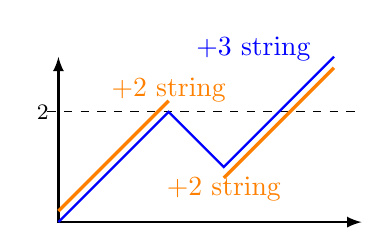
\begin{tikzpicture}[scale=.7]
                  \draw[latex-latex, thick] (0, 3) -- (0, 0) -- (5.5, 0);
                  \foreach \j in {2} {
                          \draw[dashed] (-.2, \j) -- (5.5, \j);
                          \draw (0, \j) node[left] {\footnotesize \j};
                      }
                  \draw[blue, thick] (0, 0) -- (2, 2) -- (3, 1) -- (5, 3);
                  \draw[blue] (4.75, 2.75) node[above left] {+3 string};

                  \draw[orange, very thick] (0, 0+.2) -- (2, 2+.2);
                  \draw[orange] (2,2) node[above] {+2 string};
                  \draw[orange, very thick] (3, 1-.2) -- (5, 3-.2);
                  \draw[orange] (3, 1) node[below] {+2 string};
              \end{tikzpicture}
              \caption{Decomposition of a $+3$-string into two $\pm(k+1)$-strings.}
              \label{fig:dyck_hered}
          \end{figure}
\end{itemize}

Finally, this complex algorithm has a quantum query
complexity of $O\left(\sqrt{n}(\log(n))^{0.5k}\right)$ which is a
$\tilde{\Theta}\left(\sqrt{n}\right)$. This description of the existing
algorithm stay at the surface in order to stay simple, every
subroutines' pseudo code can be found in
\autoref{annex:complete_subroutine_dyck_kn}. No proof of their
quantum query complexities are provided as a proof for
\autoref{th:subroutine_complexity}, almost identical,
is already provided in \autoref{proof:complexity_dyckkn}.
However, this algorithm can be improved, indeed the upper bound by
reduction to 2d directed grid ($O\left(\sqrt{n}(\log_2(n))^{0.5(k-1)}\right)$)
is still better than the quantum query complexity of the algorithm
($O\left(\sqrt{n}(\log_2(n))^{0.5k}\right)$).
